\documentclass{beamer}

\usepackage{stmaryrd}
\usepackage{listings}
\usepackage{graphicx}

\usepackage{euler}
%\usepackage[cm-default]{fontspec}
%\usepackage{xunicode}

%\setmainfont{Ubuntu}

\setbeamertemplate{navigation symbols}{}
\usecolortheme[rgb={0.8,0,0}]{structure}
\usefonttheme{serif}
\usefonttheme{structurebold}

\usepackage{tikz}
\usetikzlibrary{shapes.multipart}

\newenvironment{slide}[1]{\begin{frame}\frametitle{#1}}{\end{frame}}
\newenvironment{verbslide}[1]{\begin{frame}[containsverbatim]\frametitle{#1}}{\end{frame}}

\newcommand{\titlecard}[1]{\begin{frame}\begin{center}\usebeamercolor[fg]{frametitle}\usebeamerfont{frametitle}#1\end{center}\end{frame}}

\title{Introduction to Parser Combinators}
\author{Robert Atkey \newline \texttt{Robert.Atkey@cis.strath.ac.uk}}
\date{8th February 2011}

\begin{document}

\frame{\titlepage}

\section{Introduction}

\newcommand{\boundingbox}{\draw [color=white] (-5,-3) rectangle (5,3);}

\titlecard{Parsing}

\begin{frame}
  \begin{center}
    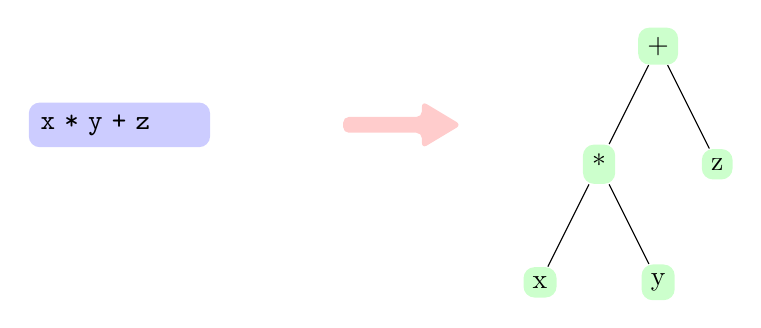
\begin{tikzpicture}
      \boundingbox

      \draw (-5,0) node[right,text width=2cm,rounded corners,fill=blue!20,inner sep=1ex]
      { \texttt{x * y + z}
      };

      \fill[color=red!20] [rounded corners=2pt] (-1,0.1) --(0,0.1) --(0,0.3) --(0.5,0) --(0,-0.3) --(0,-0.1) --(-1,-0.1) --cycle;

      \begin{scope}
        [every node/.style={fill=green!20,rounded corners}]
        \node at (3,1) {+}
        child {node {*}
          child {node {x}}
          child {node {y}}}
        child {node {z}};
      \end{scope}
    \end{tikzpicture}
  \end{center}
\end{frame}

\begin{frame}
  \begin{center}
    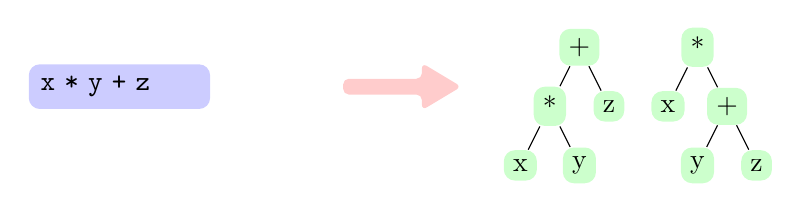
\begin{tikzpicture}
      \boundingbox

      \draw (-5,0) node[right,text width=2cm,rounded corners,fill=blue!20,inner sep=1ex]
      { \texttt{x * y + z}
      };
      
      \fill[color=red!20] [rounded corners=2pt] (-1,0.1) --(0,0.1) --(0,0.3) --(0.5,0) --(0,-0.3) --(0,-0.1) --(-1,-0.1) --cycle;

      \begin{scope}
        [every node/.style={fill=green!20,rounded corners}]

        \begin{scope}
          [scale=0.5]
          \node at (4,1) {+}
          child {node {*}
            child {node {x}}
            child {node {y}}}
          child {node {z}};

          \node at (7,1) {*}
          child {node {x}}
          child {node {+}
            child {node {y}}
            child {node {z}}};
        \end{scope}
      \end{scope}
    \end{tikzpicture}
  \end{center}
\end{frame}

\begin{frame}
  \begin{center}
    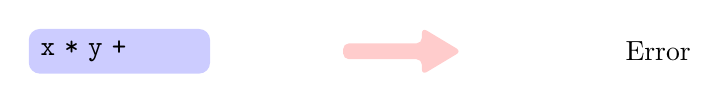
\begin{tikzpicture}
      \boundingbox

      \draw (-5,0) node[right,text width=2cm,rounded corners,fill=blue!20,inner sep=1ex]
      { \texttt{x * y + }
      };
      
      \fill[color=red!20] [rounded corners=2pt] (-1,0.1) --(0,0.1) --(0,0.3) --(0.5,0) --(0,-0.3) --(0,-0.1) --(-1,-0.1) --cycle;

      \node at (3,0)
      { Error };
    \end{tikzpicture}
  \end{center}
\end{frame}

\titlecard{Many Applications}

\begin{frame}
  \begin{center}
    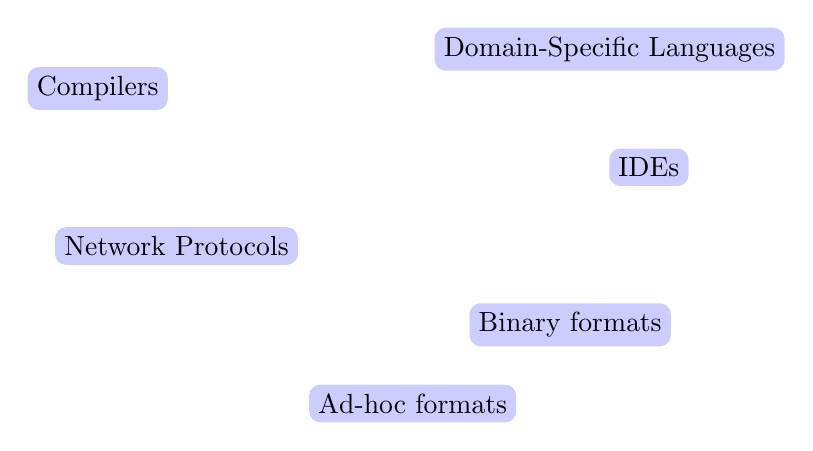
\begin{tikzpicture}
      \boundingbox

      \begin{scope}
        [every node/.style={fill=blue!20,rounded corners}]
        \node at (-4,2) { Compilers };
        \node at (3,1) { IDEs };
        \node at (2.5,2.5) { Domain-Specific Languages };
        \node at (0,-2) { Ad-hoc formats };
        \node at (-3,0) { Network Protocols };
        \node at (2,-1) { Binary formats };        
      \end{scope}
    \end{tikzpicture}
  \end{center}
\end{frame}

\titlecard{The Dream}

\begin{frame}
  \begin{center}
    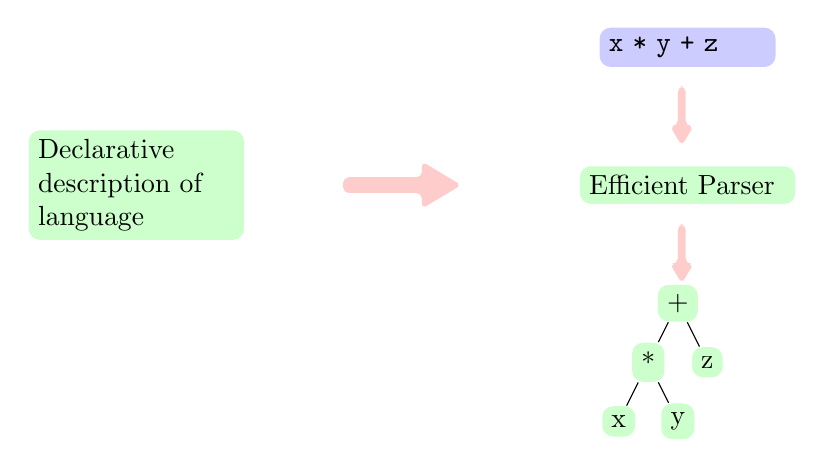
\begin{tikzpicture}
      \boundingbox

      \draw (-5,0) node[right,fill=green!20,rounded corners,text width=2.5cm]
      { Declarative \\ description of language };

      \fill[color=red!20] [rounded corners=2pt] (-1,0.1) --(0,0.1) --(0,0.3) --(0.5,0) --(0,-0.3) --(0,-0.1) --(-1,-0.1) --cycle;

      \node [right,fill=green!20,rounded corners,text width=2.5cm] at (2,0)
      { Efficient Parser };

      \node [right,fill=blue!20,rounded corners,text width=2cm] at (2.25,1.75)
      { \texttt{x * y + z} };

      \begin{scope}
        [xshift=3.3cm,yshift=0.75cm,scale=0.5,rotate=-90]
        \fill[color=red!20] [rounded corners=2pt] (-1,0.1) --(0,0.1) --(0,0.3) --(0.5,0) --(0,-0.3) --(0,-0.1) --(-1,-0.1) --cycle;
      \end{scope}

      \begin{scope}
        [xshift=3.3cm,yshift=-1cm,scale=0.5,rotate=-90]
        \fill[color=red!20] [rounded corners=2pt] (-1,0.1) --(0,0.1) --(0,0.3) --(0.5,0) --(0,-0.3) --(0,-0.1) --(-1,-0.1) --cycle;
      \end{scope}

      \begin{scope}
        [every node/.style={fill=green!20,rounded corners},scale=0.5]
        \node at (6.5,-3) {+}
        child {node {*}
          child {node {x}}
          child {node {y}}}
        child {node {z}};
      \end{scope}
    \end{tikzpicture}
  \end{center}
\end{frame}

\begin{frame}
  \begin{center}
    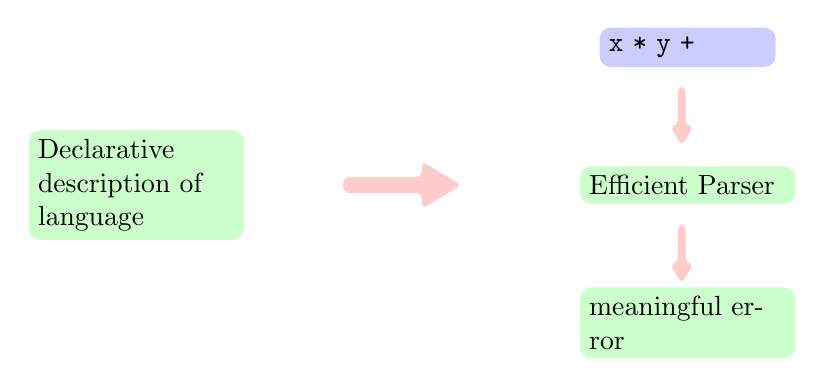
\begin{tikzpicture}
      \boundingbox

      \draw (-5,0) node[right,fill=green!20,rounded corners,text width=2.5cm]
      { Declarative \\ description of language };

      \fill[color=red!20] [rounded corners=2pt] (-1,0.1) --(0,0.1) --(0,0.3) --(0.5,0) --(0,-0.3) --(0,-0.1) --(-1,-0.1) --cycle;

      \node [right,fill=green!20,rounded corners,text width=2.5cm] at (2,0)
      { Efficient Parser };

      \node [right,fill=blue!20,rounded corners,text width=2cm] at (2.25,1.75)
      { \texttt{x * y +} };

      \begin{scope}
        [xshift=3.3cm,yshift=0.75cm,scale=0.5,rotate=-90]
        \fill[color=red!20] [rounded corners=2pt] (-1,0.1) --(0,0.1) --(0,0.3) --(0.5,0) --(0,-0.3) --(0,-0.1) --(-1,-0.1) --cycle;
      \end{scope}

      \begin{scope}
        [xshift=3.3cm,yshift=-1cm,scale=0.5,rotate=-90]
        \fill[color=red!20] [rounded corners=2pt] (-1,0.1) --(0,0.1) --(0,0.3) --(0.5,0) --(0,-0.3) --(0,-0.1) --(-1,-0.1) --cycle;
      \end{scope}

      \node [right,fill=green!20,rounded corners,text width=2.5cm] at (2,-1.75)
      { meaningful error };

      % \begin{scope}
      %   [every node/.style={fill=green!20,rounded corners},scale=0.5]
      %   \node at (6.5,-3) {+}
      %   child {node {*}
      %     child {node {x}}
      %     child {node {y}}}
      %   child {node {z}};
      % \end{scope}
    \end{tikzpicture}
  \end{center}
\end{frame}

\begin{frame}
  \begin{center}
    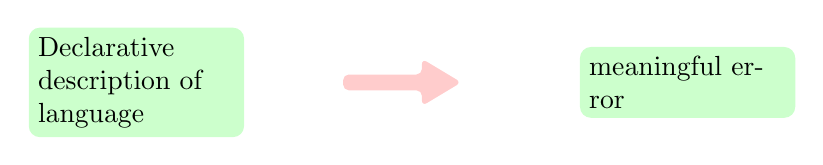
\begin{tikzpicture}
      \boundingbox

      \draw (-5,0) node[right,fill=green!20,rounded corners,text width=2.5cm]
      { Declarative \\ description of language };

      \fill[color=red!20] [rounded corners=2pt] (-1,0.1) --(0,0.1) --(0,0.3) --(0.5,0) --(0,-0.3) --(0,-0.1) --(-1,-0.1) --cycle;

      \node [right,fill=green!20,rounded corners,text width=2.5cm] at (2,0)
      { meaningful error };
    \end{tikzpicture}
  \end{center}
\end{frame}

\titlecard{The Reality}

\begin{frame}
  \begin{center}
    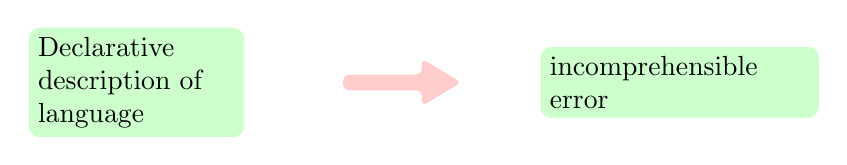
\begin{tikzpicture}
      \boundingbox

      \draw (-5,0) node[right,fill=green!20,rounded corners,text width=2.5cm]
      { Declarative \\ description of language };

      \fill[color=red!20] [rounded corners=2pt] (-1,0.1) --(0,0.1) --(0,0.3) --(0.5,0) --(0,-0.3) --(0,-0.1) --(-1,-0.1) --cycle;

      \node [right,fill=green!20,rounded corners,text width=3.3cm] at (1.5,0)
      { incomprehensible error };
    \end{tikzpicture}
  \end{center}
\end{frame}

\begin{frame}
  \begin{center}
    \begin{tikzpicture}
      \boundingbox

      \draw (-5,0) node[right,fill=green!20,rounded corners,text width=2.5cm]
      { Declarative \\ description of language };

      \fill[color=red!20] [rounded corners=2pt] (-1,0.1) --(0,0.1) --(0,0.3) --(0.5,0) --(0,-0.3) --(0,-0.1) --(-1,-0.1) --cycle;

      \node [right,fill=green!20,rounded corners,text width=2.5cm] at (2,0)
      { Efficient Parser };

      \node [right,fill=blue!20,rounded corners,text width=2cm] at (2.25,1.75)
      { \texttt{x * y + z} };

      \begin{scope}
        [xshift=3.3cm,yshift=0.75cm,scale=0.5,rotate=-90]
        \fill[color=red!20] [rounded corners=2pt] (-1,0.1) --(0,0.1) --(0,0.3) --(0.5,0) --(0,-0.3) --(0,-0.1) --(-1,-0.1) --cycle;
      \end{scope}

      \begin{scope}
        [xshift=3.3cm,yshift=-1cm,scale=0.5,rotate=-90]
        \fill[color=red!20] [rounded corners=2pt] (-1,0.1) --(0,0.1) --(0,0.3) --(0.5,0) --(0,-0.3) --(0,-0.1) --(-1,-0.1) --cycle;
      \end{scope}

      \node at (3.25,-2.2)
      { 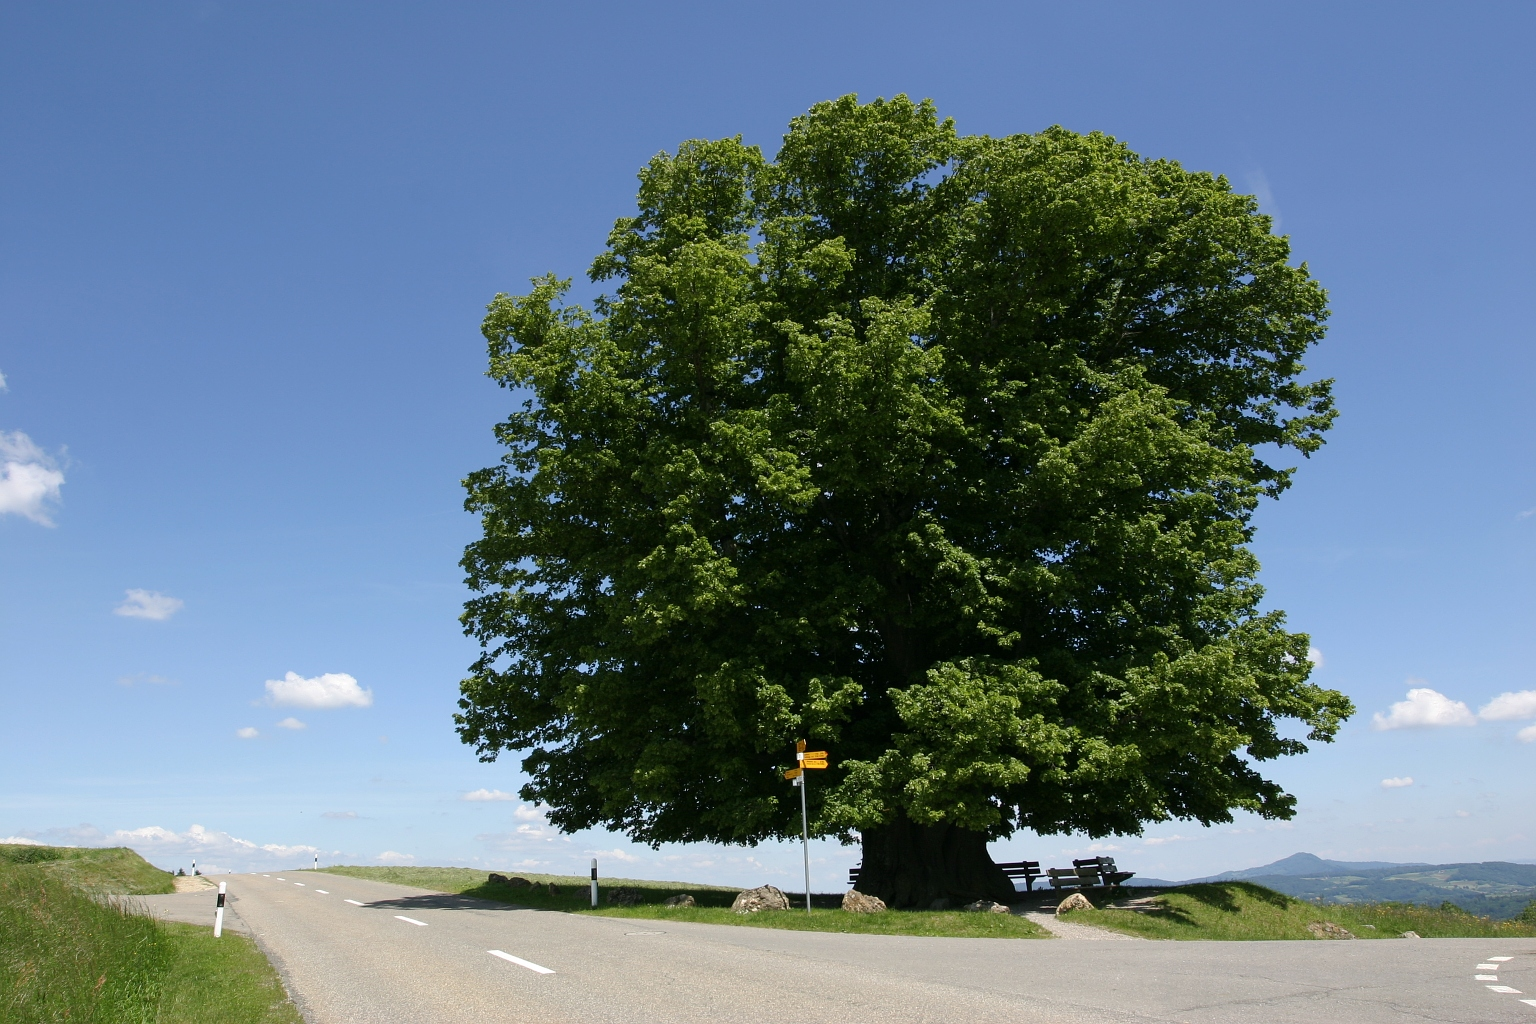
\includegraphics[width=2.5cm]{Linde_von_linn.jpg} };
    \end{tikzpicture}
  \end{center}
\end{frame}

\begin{frame}
  \begin{center}
    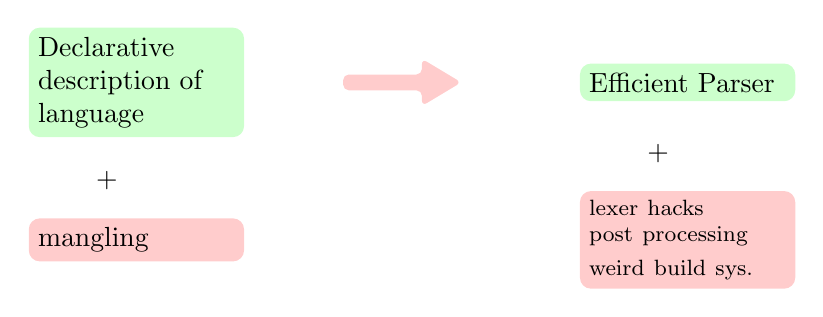
\begin{tikzpicture}
      \boundingbox

      \draw (-5,0) node[right,fill=green!20,rounded corners,text width=2.5cm]
      { Declarative \\ description of language };

      \node at (-4,-1.25) {+};

      \node [right,fill=red!20,rounded corners,text width=2.5cm] at (-5,-2)
      { mangling };

      \fill[color=red!20] [rounded corners=2pt] (-1,0.1) --(0,0.1) --(0,0.3) --(0.5,0) --(0,-0.3) --(0,-0.1) --(-1,-0.1) --cycle;

      \node [right,fill=green!20,rounded corners,text width=2.5cm] at (2,0)
      { Efficient Parser };

      \node at (3,-0.9) {+};

      \node [right,fill=red!20,rounded corners,text width=2.5cm] at (2,-2)
      { \footnotesize{lexer hacks \\ post processing \\ weird build sys. } };
    \end{tikzpicture}
  \end{center}
\end{frame}

% \titlecard{Or, write it by hand...}

% \begin{frame}[containsverbatim]
% \begin{verbatim}
% ...
% and read_additive_term env input = 
%   let t1 = read_multiplicative_term env input in
%     match input#tok with
%       | `PLUS  -> input#advance (); TF.T_binop (t1, P.Op_iadd, read_additive_term env input)
%       | `DASH  -> input#advance (); TF.T_binop (t1, P.Op_isub, read_additive_term env input)
%       | _      -> t1

% and read_multiplicative_term env input =
%   let t1 = read_base_term env input in
%     match input#tok with
%       | `STAR -> input#advance (); TF.T_binop (t1, P.Op_imul, read_multiplicative_term env input)
%       | _     -> t1
% ...
% \end{verbatim}
% \end{frame}

% \titlecard{Parser Combinators!}

% \begin{frame}
%   Toolkit for building recursive descent, top-down parsers.

%   \bigskip

%   Start with primitive parsers:
%   \begin{itemize}
%   \item \texttt{string "keyword"}, \texttt{whitespace}, \texttt{lparen}, \texttt{rparen}
%   \end{itemize}

%   \bigskip

%   Combine using \emph{combinators}:
%   \begin{itemize}
%   \item \texttt{>>=}, \texttt{<|>}, \texttt{>>}, \texttt{<\$>}, \texttt{<*>}, \texttt{many}, \texttt{some}, \texttt{sepBy}, ...
%   \end{itemize}
% \end{frame}

\section{Parser Combinators}

\titlecard{Parser Combinators}

\begin{frame}
  Parser Combinators are an
  
  \begin{itemize}
  \item[] \textbf{E}mbedded \textbf{D}omain-\textbf{S}pecific \textbf{L}anguage
  \end{itemize}
  
  (EDSL) for \emph{parsing}.

  \bigskip

  \begin{itemize}
  \item \textit{Embedded} : Inside a general-purpose language
  \item \textit{Domain-Specific} : For a specific application
  \item \textit{Language} : A means of expression
  \end{itemize}
\end{frame}

\begin{frame}
  A very small language:

  \begin{eqnarray*}
    \mathbf{exp} & ::= & \mathbf{addExp} \\
    \mathbf{addExp} & ::= & \mathbf{multExp}\ (\mathbf{ws}\ \texttt{`+'}\ \mathbf{ws}\ \mathbf{multExp})^* \\
    \mathbf{multExp} & ::= & \mathbf{basicExp}\ (\mathbf{ws}\ \texttt{`*'}\ \mathbf{ws}\ \mathbf{basicExp})^* \\
    \mathbf{basicExp} & ::= & \mathbf{number} \\
                      & | & \texttt{`('}\ \mathbf{ws}\ \mathbf{addExp}\ \mathbf{ws}\ \texttt{`)'}
  \end{eqnarray*}

  \bigskip

  Written in a DSL: Extended Backus-Naur Form (EBNF).

  \bigskip

  A string: \texttt{(12 + 67) * 89 * 123}
\end{frame}

\begin{frame}[containsverbatim]
  Translated to Parser Combinators:

\begin{verbatim}
data Exp = Num Integer | Add Exp Exp | Mul Exp Exp

exp = addExp

addExp =
  foldl Add
  <$> multExp <*> many (ws *> char '+' *> ws *> multExp)

multExp =
  foldl Mul
  <$> basicExp <*> many (ws *> char '*' *> ws *> basicExp)

basicExp =   Num <$> number
         <|> char '(' *> ws *> addExp <* ws <* char ')'
\end{verbatim}
\end{frame}

\begin{frame}[containsverbatim]
  Taking it apart:
\begin{verbatim}
addExp :: Parser Exp
addExp =
  foldl Add
  <$> multExp <*> many (ws *> char '+' *> ws *> multExp)
\end{verbatim}
  
  The bits:
  \begin{itemize}
  \item \texttt{ws} : accept whitespace, return \texttt{()}
  \item \texttt{char '+'} : accept `\texttt{+}', return \texttt{()}
  \item \texttt{*>} : sequence, ignoring LHS
  \item \texttt{many} : accept zero or more, returning a list
  \item \texttt{<*>} : sequence, apply LHS to RHS
  \item \texttt{<\$>} : transform the returned value
  \end{itemize}
\end{frame}

\begin{frame}
  Basic (very rough) idea: the type
  \begin{displaymath}
    \texttt{Parser a}
  \end{displaymath}
  represents a set of strings, tagged with (maybe many) \texttt{a} values.

  \bigskip

  \emph{Parser Combinators} are functions that generate \texttt{Parser
    a} values from existing ones, or primitive parsers.

  \bigskip

  To make it go, there is a function:
  \begin{displaymath}
    \texttt{parse :: Parser a -> String -> [a]}
  \end{displaymath}
\end{frame}

\begin{frame}
  Primitive combinators:
  \begin{eqnarray*}
    \texttt{char}  & :: & \texttt{Char -> Parser ()} \\
    \texttt{eos}   & :: & \texttt{Parser ()} \\
    \texttt{token} & :: & \texttt{Parser Char} \\
  \end{eqnarray*}

  Combinators:
  \begin{eqnarray*}
    \texttt{pure} & :: & \texttt{a -> Parser a} \\
    \texttt{<*>} & :: & \texttt{Parser (a -> b) -> Parser a -> Parser b} \\
    \texttt{<|>} & :: & \texttt{Parser a -> Parser a -> Parser a} \\
    \texttt{empty} & :: & \texttt{Parser a}
  \end{eqnarray*}

  \bigskip

  \texttt{Parser} is \texttt{Applicative} and \texttt{Alternative}.

  \bigskip

  Plus the ``forgotten'' combinator: recursion.
\end{frame}

\begin{frame}[containsverbatim]
  Derived Combinators:
  \begin{eqnarray*}
    \texttt{<\$>}   & :: & \texttt{(a -> b) -> Parser a -> Parser b} \\
    \texttt{*>}     & :: & \texttt{Parser a -> Parser b -> Parser b} \\
    \texttt{many}   & :: & \texttt{Parser a -> Parser [a]} \\
    \texttt{some}   & :: & \texttt{Parser a -> Parser [a]} \\
    \texttt{ws}     & :: & \texttt{Parser ()} \\
    \texttt{number} & :: & \texttt{Parser Integer}
  \end{eqnarray*}

  \bigskip

  For example:
\begin{verbatim}
many :: Parser a -> Parser [a]
many p = (:) <$> p <*> many p
         <|>
         pure []
\end{verbatim}
\end{frame}

\begin{frame}[containsverbatim]
  The combinators so far have not allowed the language being parsed to
  depend on the input.

  \bigskip

  For example, to parse well-formed XML we must enforce the constraint
  that open tags and close tags match:
\begin{verbatim}
<rant>
  In my day, we made parsers with yacc, and we liked it.
  ...
</rant>
\end{verbatim}

  \bigskip

  A parser:
\begin{verbatim}
element = Elem <$> openTag <*> nodes <*> closeTag
\end{verbatim}
  No way for \texttt{openTag} to communicate to \texttt{closeTag} what
  name to expect.
\end{frame}

\begin{frame}[containsverbatim]
  To introduce context-sensitivity, we add some new basic combinators:
  \begin{eqnarray*}
    \texttt{return} & :: & \texttt{a -> Parser a} \\
    \texttt{>>=}    & :: & \texttt{Parser a -> (a -> Parser b) -> Parser b}
  \end{eqnarray*}

  \bigskip

  \texttt{return} is the same thing as \texttt{pure}.

  \bigskip

  \texttt{>>=} (``bind'') is very powerful:
\begin{verbatim}
element = openTag          >>= \tagName ->
          nodes            >>= \ns ->
          closeTag tagName >>= \_ ->
          return (Elem tagName ns)
\end{verbatim}
\end{frame}

\begin{frame}[containsverbatim]
  But this looks ghastly!

  \bigskip

  Sweeten with sugar:
\begin{verbatim}
element = do tagName <- openTag
             ns <- nodes
             closeTag tagName
             return (Elem tagName ns)
\end{verbatim}

  \bigskip

  \texttt{Parser} is a \texttt{Monad}.
\end{frame}

\section{(An) Implementation}

\titlecard{(An) Implementation}

\begin{frame}[containsverbatim]
  Let us implement:
\begin{verbatim}
type Parser a = String -> [(a,String)]
\end{verbatim}

  \bigskip

  Idea: if \texttt{p :: Parser a} tags the string \texttt{s} with the
  value \texttt{x}, then \texttt{(x,s')} is a member of \texttt{p (s
    ++ s')}. (Roughly; one also needs to define what happens for EOS).

  \bigskip

  In other words, \texttt{p s} returns all the possible parses of
  prefixes of \texttt{s} with the remaining string and value.
\end{frame}

\begin{frame}[containsverbatim]
  Primitive parsers:
\begin{verbatim}
token :: Parser Char
token ""     = []
token (c:cs) = [(c,cs)]

eos :: Parser ()
eos "" = [((),"")]
eos _  = []

char :: Char -> Parser ()
char c ""      = []
char c (c':cs) = if c == c' then [((),cs)] else []
\end{verbatim}
\end{frame}

\begin{frame}[containsverbatim]
  Combinators:
\begin{verbatim}
return :: a -> Parser a
return a cs = [(a,cs)]

(>>=) :: Parser a -> (a -> Parser b) -> Parser b
(p >>= f) cs = concatMap (\(a,cs') -> f a cs') (p cs)

concatMap :: (a -> [b]) -> [a] -> [b]

empty :: Parser a
empty = []

(<|>) :: Parser a -> Parser a -> Parser a
(p1 <|> p2) cs = p1 cs ++ p2 cs
\end{verbatim}
\end{frame}

\begin{frame}[containsverbatim]
  Other definitions:

\begin{verbatim}
(<*>) :: Parser (a -> b) -> Parser a -> Parser b
p1 <*> p2 = do f <- p1
               a <- p2
               return (f a)
\end{verbatim}

\bigskip

In a real implementation, once we tell Haskell that \texttt{Parser} is
an \texttt{Applicative}, \texttt{Alternative} and \texttt{Monad}, then
lots of stuff comes for free: \texttt{many}, \texttt{some},
\texttt{*>}, ...
  
\end{frame}

\section{That's Great! What More Could We Want?}

\titlecard{That's Great! What More Could We Want?}

\begin{frame}
  Problems with this implementation:
  \begin{itemize}
  \item Slow: mainly due to list concatenation
  \item Returns many results
  \item Non-existent error reporting
  \item Space leak on long inputs
  \item Only parses strings
  \item Only parses in-memory data (sort of)
  \end{itemize}
\end{frame}

% \section{Classical Parser Combinators}

% \titlecard{Classical Combinator Parsers}

% \begin{frame}
%   A type constructor: \texttt{Parser :: * -> *}

%   \bigskip

%   \begin{itemize}
%   \item \texttt{Parser Integer} - parsers that return integers
%   \item \texttt{Parser Exp} - parsers that return expressions
%   \item \texttt{Parser [Exp]} - parsers that return lists of expressions
%   \end{itemize}
  
%   \bigskip

%   \texttt{parse :: Parser a -> String -> [(a,String)]}

%   % \bigskip

%   % \texttt{Parser a} is a recursive descent parser that yields values
%   % of type \texttt{a}.
% \end{frame}

% \titlecard{Primitive Parsers}

% \begin{frame}
%   \begin{itemize}
%   \item \texttt{digit :: Parser Integer}
%   \item \texttt{number :: Parser Integer}
%   \item \texttt{whitespace :: Parser ()}
%   \item \texttt{char :: Char -> Parser ()}
%   \item \texttt{string :: String -> Parser ()}
%   \item \texttt{comma :: Parser ()}
%   \end{itemize}
% \end{frame}

% \titlecard{Combinators}

% \begin{frame}
%   \frametitle{Sequencing}

%   \begin{itemize}
%   \item \texttt{>>= :: Parser a -> (a -> Parser b) -> Parser b}
%   \item \texttt{return :: a -> Parser a}
%   \end{itemize}

%   \bigskip

%   \texttt{Parser} is a \emph{monad}.

%   \bigskip

%   Syntactic sugar for monads (\texttt{do}-notation):

%   \begin{displaymath}
%     \begin{array}{rcl}
%       \texttt{do x <- e1; e2} & \Rightarrow & \texttt{e1 >>= ($\lambda$x -> e2)}
%     \end{array}
%   \end{displaymath}
% \end{frame}

% \begin{frame}
%   \frametitle{Choice, Alternatives}

%   \begin{itemize}
%   \item \texttt{empty :: Parser a}
%   \item \texttt{(<|>) :: Parser a -> Parser a -> Parser a}
%   \end{itemize}
% \end{frame}

% \titlecard{An Example}

% \begin{slide}{Functors}
%   \begin{itemize}
%   \item \texttt{fmap :: (a -> b) -> Parser a -> Parser b}
%   \end{itemize}

%   \bigskip

%   Also available in infix: \\
%   \quad\quad\texttt{<\$> :: (a -> b) -> Parser a -> Parser b}
% \end{slide}

% \begin{slide}{Applicative Functors}
%   \begin{itemize}
%   \item \texttt{pure :: a -> Parser a}
%   \item \texttt{<*> :: Parser (a -> b) -> Parser a -> Parser b}
%   \end{itemize}
% \end{slide}

% \titlecard{Applicative Functor Example}

% \titlecard{Context Sensitivity}

% \titlecard{Inside the Machine}

% \begin{slide}{Sources of Inefficiency}
%   \begin{itemize}
%   \item Excessive use of list concatenation
%   \item Unrestricted backtracking
%   \item Returning multiple parses
%   \item Space leaks
%   \end{itemize}
% \end{slide}

\begin{verbslide}{}
  Change implementation to:
\begin{verbatim}
type Parser a = String -> Maybe (a, String)
\end{verbatim}

  \bigskip

  When looking at alternatives:
  \begin{displaymath}
    \texttt{p <|> q}
  \end{displaymath}
  Only try \texttt{q} if \texttt{p} fails.
\end{verbslide}

\begin{slide}{}
  \begin{enumerate}
  \item Localise backtracking:
    \begin{displaymath}
      \texttt{(p <|> q) >>= f}
    \end{displaymath}
    decide, once and for all, which one of \texttt{p} or \texttt{q}
    will be used before doing \texttt{f}.
  \item Prolog-style cut combinator: \texttt{commit :: Parser a}
  \item Limited lookahead:
    \begin{displaymath}
      \texttt{p <|> q}
    \end{displaymath}
    Only try \texttt{q} if \texttt{p} fails \emph{without consuming
      any input}.
    \begin{itemize}
    \item Add \texttt{try :: Parser a -> Parser a} that pretends to
      not consume input on failure.
    \end{itemize}
  \item Trying all alternatives in ``parallel''.
  \end{enumerate}
\end{slide}

\begin{slide}{}
  \begin{itemize}
  \item Error reporting:
    \begin{itemize}
    \item Add \texttt{<?> :: Parser a -> String -> Parser a}
    \item Track position information
    \end{itemize}
  \item Error correction:
    \begin{itemize}
    \item Insertion/deletion of tokens
    \item Requires much more sophisticated implementation
    \end{itemize}
  \item Incremental Input:
    \begin{itemize}
    \item \emph{Don't use lazy IO!}
    \item Feed in input in chunks, parser must be able to “suspend”
    \end{itemize}
  \item Incremental Output:
    \begin{itemize}
    \item Start producing output before end of input
    \item Not clear what this means; not commonly implemented
    \end{itemize}
  \end{itemize}
\end{slide}

\titlecard{Advantages of Parser Combinators}

\begin{frame}
  \begin{itemize}
  \item Hackable
    \begin{itemize}
    \item (Generally) Simple recusive descent algorithm
    \item Easy to understand
    \item Easy to tweak
    \item Easy access to context-sensitivity
    \end{itemize}
  \item No code generation step
  \item Looks a lot like a real grammar
  \item Construct parsers on the fly
  \item Can be “scannerless”
  \item Can be efficient (usually)
  \item Mature implementations (Parsec, Attoparsec)
  \end{itemize}
\end{frame}

\titlecard{Disadvantages of Parser Combinators}

\begin{frame}
  \begin{itemize}
  \item No time or space guarantees
    \begin{itemize}
    \item E.g.: $O(n)$ for LL/LR/PEG parsers, $O(n^3)$ for general context-free
    \end{itemize}
  \item All you can do is parse:
    \begin{itemize}
    \item No grammar analysis
    \item No pretty printing
    \item No graphical tools for debugging
    \item No generation
    \end{itemize}
  \item No left-recursion (apart from one implementation)
  \item Sometimes odd behaviour when parsing alternatives
  \item Every library has subtly different behaviour
  \end{itemize}
\end{frame}

\titlecard{Some Haskell Implementations}

\begin{frame}
  \begin{itemize}
  \item Parsec (2 and 3)
    \begin{itemize}
    \item Version 2 included in Haskell platform
    \item ``Industrial Strength''
    \item Lots of derived parsers for tokens, expressions, permutations
    \item Uses localised backtracking, limited lookahead + \texttt{try}
    \item Tracks positions, good error reporting
    \end{itemize}
  \item Attoparsec:
    \begin{itemize}
    \item Designed for binary protocols: \texttt{ByteString} input
    \item Careful implementation for speed
    \item Limited error reporting (no source positions)
    \item Incremental input
    \end{itemize}
  \item polyparse:
    \begin{itemize}
    \item Uses \texttt{commit} for backtracking control
    \end{itemize}
  \item UU-Parsinglib:
    \begin{itemize}
    \item Advanced set of error-correcting combinators
    \item Big set of derived combinators.
    \end{itemize}
  \end{itemize}

  \bigskip

  \tiny{Other parser combinator libraries (for other languages) are available.}
\end{frame}

\begin{frame}
  Some references:

  \bigskip

  Graham Hutton and Erik Meijer. \emph{Monadic Parsing in
    Haskell}. Journal of Functional Programming, 8(4):437--444, 1998.

  \bigskip

  Graham Hutton and Erik Meijer. \emph{Monadic parser
    combinators}. Technical Report NOTTCS-TR-96-4, Dept. Computer
  Science, University of Nottingham, 1996.

  \bigskip

  Peter Ljungl\"of. \emph{Pure Functional Parsing - an advanced
    tutorial}. Licenciate thesis, Department of Computer Science,
  Gothenburg University and Chalmers University of Technology, April
  2002.
\end{frame}

\begin{frame}
  Picture credits:
  \begin{itemize}
  \item \url{http://commons.wikimedia.org/wiki/File:Linde_von_linn.jpg} by Stefan Wernli \\
     Creative Commons Attribution-Share Alike 2.5 Generic
  \end{itemize}

  \begin{center}
    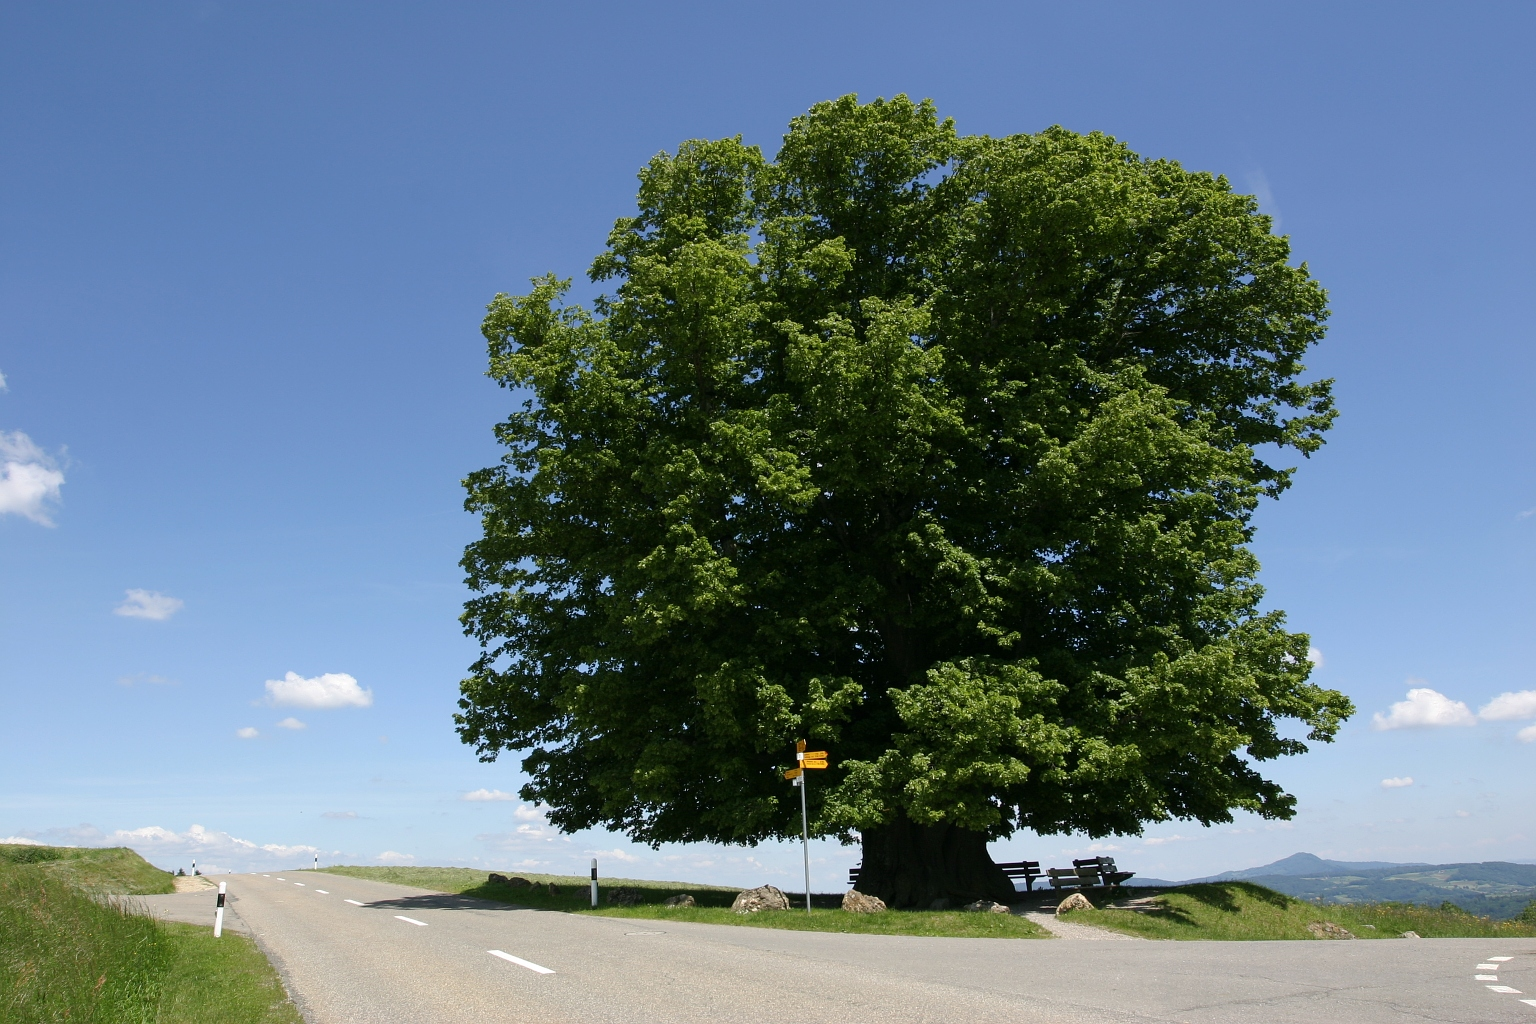
\includegraphics[width=5cm]{Linde_von_linn.jpg}    
  \end{center}
\end{frame}

\end{document}
